\documentclass{vkr}
\usepackage[english, russian]{babel} % переносы
\usepackage{graphicx} % для вставки картинок
\graphicspath{{images/}} % путь к изображениям
\usepackage[hidelinks]{hyperref}
\usepackage{float} % определяет метод H для рисунка с переносом на следующую страницу, ели не помещается
\usepackage{pdflscape}
\addto{\captionsrussian}{\renewcommand{\refname}{СПИСОК ИСПОЛЬЗОВАННЫХ ИСТОЧНИКОВ}}
\usepackage{xltabular} % для вставки таблиц
\usepackage{makecell}
\renewcommand\theadfont{} % шрифт в /thead
\usepackage{array} % для определения новых типов столбцов таблиц
\newcolumntype{T}{>{\centering\arraybackslash}X} % новый тип столбца T - автоматическая ширина столбца с выравниванием по центру
\newcolumntype{R}{>{\raggedleft\arraybackslash}X} % новый тип столбца R - автоматическая ширина столбца с выравниванием по правому краю
\newcolumntype{C}[1]{>{\centering\let\newline\\\arraybackslash\hspace{0pt}}m{#1}} % новый тип столбца C - фиксированная ширина столбца с выравниванием по центру
\newcolumntype{r}[1]{>{\raggedleft\arraybackslash}p{#1}} % новый тип столбца r - фиксированная ширина столбца с выравниванием по правому краю
\newcommand{\centrow}{\centering\arraybackslash} % командой \centrow можно центрировать одну ячейку (заголовок) в столбце типа X или p, оставив в оcтальных ячейках другой тип выравнивания
\newcommand{\finishhead}{\endhead\hline\endlastfoot}
\newcommand{\continuecaption}[1]{\caption*{#1}\\ \hline }
\usepackage{etoolbox}
\AtBeginEnvironment{xltabular}{\refstepcounter{tablecnt}} % подсчет таблиц xltabular, обычные таблицы подсчитываются в классе

\usepackage[tableposition=top]{caption} % подпись таблицы вверху
\captionsetup{strut=off}
\setlength{\intextsep}{0pt} % Vertical space above & below [h] floats
\setlength{\textfloatsep}{0pt} % Vertical space below (above) [t] ([b]) floats
\DeclareCaptionLabelFormat{gostfigure}{Рисунок #2} %подпись рисунка
\DeclareCaptionLabelFormat{gosttable}{Таблица #2} %подпись таблицы
\DeclareCaptionLabelSeparator{gost}{~--~} %разделитель в рисунках и таблицах
\captionsetup{labelsep=gost}
\captionsetup[figure]{aboveskip=10pt,belowskip=4mm,justification=centering,labelformat=gostfigure} % настройка подписи рисунка
\captionsetup[table]{font={stretch=1.41},skip=0pt,belowskip=0pt,aboveskip=8.5pt,singlelinecheck=off,labelformat=gosttable} % настройка подписи таблицы

\setlength{\LTpre}{8mm} % отступ сверху таблицы
\setlength{\LTpost}{6mm} % отступ снизу таблицы

\usepackage{enumitem}
\setlist{nolistsep,wide=\parindent,itemindent=*} % отступы вокруг списков, выравнивание с учетом разделителя

\usepackage{color} %% это для отображения цвета в коде
\usepackage{listings} %% листинги кода
\setmonofont[Scale=0.7]{Verdana} % моноширный шрифт для листинга

\definecolor{codegreen}{rgb}{0,0.6,0}
\definecolor{codegray}{rgb}{0.5,0.5,0.5}
\definecolor{codepurple}{rgb}{0.58,0,0.82}

\lstset{ %
language=C,                 % выбор языка для подсветки (здесь это С)
numbers=left,               % где поставить нумерацию строк (слева\справа)
numberstyle=\tiny,           % размер шрифта для номеров строк
stepnumber=1,                   % размер шага между двумя номерами строк
numbersep=5pt,                % как далеко отстоят номера строк от подсвечиваемого кода
commentstyle=\color{codegreen},
keywordstyle=\color{magenta},
numberstyle=\tiny\color{codegray},
stringstyle=\color{codepurple},
basicstyle=\linespread{0.95}\ttfamily,
backgroundcolor=\color{white}, % цвет фона подсветки - используем \usepackage{color}
showspaces=false,            % показывать или нет пробелы специальными отступами
showstringspaces=false,      % показывать или нет пробелы в строках
showtabs=false,             % показывать или нет табуляцию в строках
frame=single,              % рисовать рамку вокруг кода
tabsize=2,                 % размер табуляции по умолчанию равен 2 пробелам
captionpos=t,              % позиция заголовка вверху [t] или внизу [b] 
breaklines=true,           % автоматически переносить строки (да\нет)
breakatwhitespace=false, % переносить строки только если есть пробел
escapeinside={\%*}{*)}   % если нужно добавить комментарии в коде
}

\makeatletter % чтобы допускались русские комментарии в листингах
\lst@InputCatcodes
\def\lst@DefEC{%
 \lst@CCECUse \lst@ProcessLetter
  ^^80^^81^^82^^83^^84^^85^^86^^87^^88^^89^^8a^^8b^^8c^^8d^^8e^^8f%
  ^^90^^91^^92^^93^^94^^95^^96^^97^^98^^99^^9a^^9b^^9c^^9d^^9e^^9f%
  ^^a0^^a1^^a2^^a3^^a4^^a5^^a6^^a7^^a8^^a9^^aa^^ab^^ac^^ad^^ae^^af%
  ^^b0^^b1^^b2^^b3^^b4^^b5^^b6^^b7^^b8^^b9^^ba^^bb^^bc^^bd^^be^^bf%
  ^^c0^^c1^^c2^^c3^^c4^^c5^^c6^^c7^^c8^^c9^^ca^^cb^^cc^^cd^^ce^^cf%
  ^^d0^^d1^^d2^^d3^^d4^^d5^^d6^^d7^^d8^^d9^^da^^db_info^^dc^^dd^^de^^df%
  ^^e0^^e1^^e2^^e3^^e4^^e5^^e6^^e7^^e8^^e9^^ea^^eb^^ec^^ed^^ee^^ef%
  ^^f0^^f1^^f2^^f3^^f4^^f5^^f6^^f7^^f8^^f9^^fa^^fb^^fc^^fd^^fe^^ff%
  ^^^^20ac^^^^0153^^^^0152%
  % Basic Cyrillic alphabet coverage
  ^^^^0410^^^^0411^^^^0412^^^^0413^^^^0414^^^^0415^^^^0416^^^^0417%
  ^^^^0418^^^^0419^^^^041a^^^^041b^^^^041c^^^^041d^^^^041e^^^^041f%
  ^^^^0420^^^^0421^^^^0422^^^^0423^^^^0424^^^^0425^^^^0426^^^^0427%
  ^^^^0428^^^^0429^^^^042a^^^^042b^^^^042c^^^^042d^^^^042e^^^^042f%
  ^^^^0430^^^^0431^^^^0432^^^^0433^^^^0434^^^^0435^^^^0436^^^^0437%
  ^^^^0438^^^^0439^^^^043a^^^^043b^^^^043c^^^^043d^^^^043e^^^^043f%
  ^^^^0440^^^^0441^^^^0442^^^^0443^^^^0444^^^^0445^^^^0446^^^^0447%
  ^^^^0448^^^^0449^^^^044a^^^^044b^^^^044c^^^^044d^^^^044e^^^^044f%
  ^^^^0401^^^^0451%
  %%%
  ^^00}
\lst@RestoreCatcodes
\makeatother


% Режим шаблона (должен быть включен один из трех)
%\ВКРtrue
%\Практикаtrue
\Курсоваяtrue

\newcommand{\Дисциплина}{<<Проектирование и архитектура программных систем>>} % для курсовой
\newcommand{\КодСпециальности}{09.03.04} % Курсовая
\newcommand{\Специальность}{Программная инженерия} % Курсовая
\newcommand{\Тема}{Разработка web-сайта «Русатом – Аддитивные технологии» на платформе} % ВКР Курсовая
\newcommand{\ТемаВтораяСтрока}{1С-Битрикс}
\newcommand{\ГдеПроводитсяПрактика}{Юго-Западном государственном университете} % для практики
\newcommand{\РуководительПрактПредпр}{Куркина А. В.} % для практики
\newcommand{\ДолжнРуководительПрактПредпр}{директор} % для практики
\newcommand{\РуководительПрактУнивер}{Чаплыгин А. А.} % для практики
\newcommand{\ДолжнРуководительПрактУнивер}{к.т.н. доцент} % для практики
\newcommand{\Автор}{А. В. Тарасов}
\newcommand{\АвторРод}{Тарасова А.В.}
\newcommand{\АвторПолностьюРод}{Тарасова Артема Вячеславовича} % для практики
\newcommand{\Шифр}{хх-хх-хххх}
\newcommand{\Курс}{3} % для практики
\newcommand{\Группа}{ПО-11б}
\newcommand{\Руководитель}{А. А. Чаплыгин} % для ВКР и курсовой
\newcommand{\Нормоконтроль}{А. А. Чаплыгин} % для ВКР
\newcommand{\ЗавКаф}{А. В. Малышев} % для ВКР
\newcommand{\ДатаПриказа}{«07» апреля 2023~г.} % для ВКР
\newcommand{\НомерПриказа}{1505-с} % для ВКР
\newcommand{\СрокПредоставления}{«13» июня 2023~г.} % для ВКР, курсового

\begin{document}
\maketitle
\ifПрактика{}\else{
   \newpage
\begin{center}
\large\textbf{Минобрнауки России}

\large\textbf{Юго-Западный государственный университет}
\vskip 1em
\normalsize{Кафедра программной инженерии}
\vskip 1em
\ifВКР{
        \begin{flushright}
        \begin{tabular}{p{.4\textwidth}}
        \centrow УТВЕРЖДАЮ: \\
        \centrow Заведующий кафедрой \\
        \hrulefill \\
        \setarstrut{\footnotesize}
        \centrow\footnotesize{(подпись, инициалы, фамилия)}\\
        \restorearstrut
        «\underline{\hspace{1cm}}»
        \underline{\hspace{3cm}}
        20\underline{\hspace{1cm}} г.\\
        \end{tabular}
        \end{flushright}
        }\fi
\end{center}
\vspace{1em}
  \begin{center}
  \large
\ifВКР{
ЗАДАНИЕ НА ВЫПУСКНУЮ КВАЛИФИКАЦИОННУЮ РАБОТУ
  ПО ПРОГРАММЕ БАКАЛАВРИАТА}
  \else
ЗАДАНИЕ НА КУРСОВУЮ РАБОТУ (ПРОЕКТ)
\fi
\normalsize
  \end{center}
\vspace{1em}
{\parindent0pt
  Студента \АвторРод, шифр\ \Шифр, группа \Группа
  
1. Тема «\Тема\ \ТемаВтораяСтрока»
\ifВКР{
утверждена приказом ректора ЮЗГУ от \ДатаПриказа\ № \НомерПриказа
}\fi.

2. Срок предоставления работы к защите \СрокПредоставления

3. Исходные данные для создания программной системы:

3.1. Перечень решаемых задач:}

\renewcommand\labelenumi{\theenumi)}

\begin{enumerate}
\item проанализировать основные критерии эффективного онлайн-портфолио;
\item разработка концептуальной модели веб-сайта портфолио;
\item программную систему управления веб-портфолио;
\item сконструировать и протестировать  веб-сайт портфолио фотографа;
\end{enumerate}

{\parindent0pt
  3.2. Входные данные и требуемые результаты для программы:}

\begin{enumerate}
\item Входными данными для веб-сайта портфолио фотографа являются: изображения и фотографии в высоком разрешении для создания портфолио, описание работ, включая дополнительные детали, метаданные и контекст, дизайнерские предпочтения и требования к визуальной составляющей веб-сайта.
\item Выходными данными для программной системы являются: сформированные страницы портфолио с изображениями и описаниями работ, запросы и формы обратной связи для потенциальных клиентов, сведения о выполненных работах, визуальные отчеты о статусе и активности портфолио.
\end{enumerate}

{\parindent0pt

  4. Содержание работы (по разделам):
  
  4.1. Введение
  
  4.1. Анализ предметной области
  
4.2. Техническое задание: основание для разработки, назначение разработки,
требования к программной системе, требования к оформлению документации.

4.3. Технический проект: общие сведения о программной системе, проект
данных программной системы, проектирование архитектуры программной системы, проектирование пользовательского интерфейса программной системы.

4.4. Рабочий проект: спецификация компонентов и классов программной системы, тестирование программной системы, сборка компонентов программной системы.

4.5. Заключение

4.6. Список использованных источников

5. Перечень графического материала:

\списокПлакатов

\vskip 2em
\begin{tabular}{p{6.8cm}C{3.8cm}C{4.8cm}}
Руководитель \ifВКР{ВКР}\else работы (проекта) \fi & \lhrulefill{\fill} & \fillcenter\Руководитель\\
\setarstrut{\footnotesize}
& \footnotesize{(подпись, дата)} & \footnotesize{(инициалы, фамилия)}\\
\restorearstrut
Задание принял к исполнению & \lhrulefill{\fill} & \fillcenter\Автор\\
\setarstrut{\footnotesize}
& \footnotesize{(подпись, дата)} & \footnotesize{(инициалы, фамилия)}\\
\restorearstrut
\end{tabular}
}

\renewcommand\labelenumi{\theenumi.}

   \abstract{РЕФЕРАТ}

Объем работы равен \formbytotal{lastpage}{страниц}{е}{ам}{ам}. Работа содержит \formbytotal{figurecnt}{иллюстраци}{ю}{и}{й}, \formbytotal{tablecnt}{таблиц}{у}{ы}{}, \arabic{bibcount} библиографических источников и \formbytotal{числоПлакатов}{лист}{}{а}{ов} графического материала. Количество приложений – 2. Графический материал представлен в приложении А. Фрагменты исходного кода представлены в приложении Б.

Перечень ключевых слов: коммерческий сайт, Система, CMS, Битрикс, Joomla, аддитивные технологии, 3D-принтеры, услуги, сервисы, информатизация, автоматизация, информационные технологии, веб-форма,  Apache, классы, база данных, средства защиты информации, подсистема, компонент, модуль, сущность, информационный блок, метод, контент-редактор, администратор, пользователь, web-сайт.

Объектом разработки является web-сайт компании,  занимающейся производством 3D-принтеров, выпуском оборудования для создания порошков, разработкой программного обеспечения и организацией центров аддитивного производства.

Целью выпускной квалификационной работы является привлечение клиентов, увеличение заказов, информирование о продукции и услугах путем создания сайта компании.

В процессе создания сайта были выделены основные сущности путем создания информационных блоков, использованы классы и методы модулей, обеспечивающие работу с сущностями предметной области, а также корректную работу web-сайта, разработаны разделы, содержащие информацию о компании, ее деятельности, производимой продукции и услугах, разработан сервис по заказу 3D-деталей.

При разработке сайта использовалась система управления контентом "<1С-Битрикс: Управление сайтом">.

Разработанный сайт был успешно внедрен в компании.

\selectlanguage{english}
\abstract{ABSTRACT}
  
The volume of work is \formbytotal{lastpage}{page}{}{s}{s}. The work contains \formbytotal{figurecnt}{illustration}{}{s}{s}, \formbytotal{tablecnt}{table}{}{s}{s}, \arabic{bibcount} bibliographic sources and \formbytotal{числоПлакатов}{sheet}{}{s}{s} of graphic material. The number of applications is 2. The graphic material is presented in annex A. The layout of the site, including the connection of components, is presented in annex B.

List of keywords: commercial website, System, CMS, Bitrix, Joomla, additive technologies, 3D printers, services, services, informatization, automation, information technology, web form, Apache, classes, database, component, module, entity, information block, method, content editor, administrator, user, web site.

The object of the research is the analysis of information technologies for the development of a production company's website.

The object of the development is the website of a company engaged in the production of 3D printers, the production of equipment for the creation of powders, software development and the organization of additive manufacturing centers.

The purpose of the final qualifying work is to attract customers, increase orders, inform about products and services by creating a company website.

In the process of creating the site, the main entities were identified by creating information blocks, classes and methods of modules were used to ensure work with the entities of the subject area, as well as the correct operation of the website, sections containing information about the company, its activities, products and services were developed, a service for ordering 3D parts was developed.

When developing the site, the content management system <<1C – Bitrix: Site Management>> was used.

The developed website was successfully implemented in the company.
\selectlanguage{russian}
}\fi
\tableofcontents
\section*{ОБОЗНАЧЕНИЯ И СОКРАЩЕНИЯ}

БД -- база данных.

ИС -- информационная система.

ИТ -- информационные технологии. 

КТС -- комплекс технических средств.

ОМТС -- отдел материально-технического снабжения. 

ПО -- программное обеспечение.

РП -- рабочий проект.

СУБД -- система управления базами данных.

ТЗ -- техническое задание.

ТП -- технический проект.

UML (Unified Modelling Language) -- язык графического описания для объектного моделирования в области разработки программного обеспечения.

\ifПрактика{}\else{\section*{ВВЕДЕНИЕ}
\addcontentsline{toc}{section}{ВВЕДЕНИЕ}

Аддитивные технологии (АТ) начали активно развиваться со времени получения первых трехмерных изображений изделий на дисплеях компьютеров. Начало положила стереолитография, затем довольно многочисленные новые принципы стали называть технологиями быстрого прототипирования, затем укоренилось название "<Аддитивные технологии">. Интенсивность развития данных технологий не имеет аналогов. АТ изменили процессы проектирования и конструирования изделий, превратив их в процессы непрерывного создания изделий. Современные проектирование и производство изделий невозможно представить без данного рода технологий. 3D-принтеры стали такими же распространенными, как и персональные компьютеры. С помощью 3D-принтеров получают ткани, обувь, продукты питания, а также выращивают человеческие органы. Во многих отраслях, например, в космической отрасли, альтернативы аддитивным технологиям нет.

АТ предполагают изготовление детали методом послойного нанесения материала, в отличие от традиционных методов формирования детали, за счёт удаления материала из массива заготовки.

При использовании АТ все стадии реализации проекта от идеи до материализации находятся в единой технологической цепи, в которой каждая технологическая операция выполняется в цифровой CAD/CAM/CAE-системе.

Современные компании, видя, как развиваются информационные технологии, пытаются использовать их выгодно для своего бизнеса, поэтому запускают свой web-сайт. С его помощью предприятие может заявить о себе, проинформировать потенциального заказчика об услугах или продуктах, которые предоставляет, а также позволяет пользователям сделать с помощью сайта онлайн-заказ, произвести покупку или оплатить счета.

Сайт считается лицом компании и может существенно повысить ее имидж. Любой пользователь сети Интернет сможет получить необходимую информацию о компании в любой момент, появляется возможность найти контактные телефоны, адрес и e-mail, чтобы связаться с компанией. Сейчас большинство клиентов узнают о ее существовании именно через сайт. Поэтому сайт можно назвать самой лучшей рекламой. 

Главной задачей профессионально построенного сайта является превращение посетителя, зашедшего на сайт, в потенциального клиента.

\emph{Цель настоящей работы} – разработка web-сайта компании для привлечения новой аудитории, увеличения заказов, рекламы продукции и услуг компании. Для достижения поставленной цели необходимо решить \emph{следующие задачи:}
\begin{itemize}
\item провести анализ предметной области;
\item разработать концептуальную модель web-сайта;
\item спроектировать web-сайт;
\item реализовать сайт средствами web-технологий.
\end{itemize}

\emph{Структура и объем работы.} Отчет состоит из введения, 4 разделов основной части, заключения, списка использованных источников, 2 приложений. Текст выпускной квалификационной работы равен \formbytotal{page}{страниц}{е}{ам}{ам}.

\emph{Во введении} сформулирована цель работы, поставлены задачи разработки, описана структура работы, приведено краткое содержание каждого из разделов.

\emph{В первом разделе} на стадии описания технической характеристики предметной области приводится сбор информации о деятельности компании, для которой осуществляется разработка сайта.

\emph{Во втором разделе} на стадии технического задания приводятся требования к разрабатываемому сайту.

\emph{В третьем разделе} на стадии технического проектирования представлены проектные решения для web-сайта.

\emph{В четвертом разделе} приводится список классов и их методов, использованных при разработке сайта, производится тестирование разработанного сайта.

В заключении излагаются основные результаты работы, полученные в ходе разработки.

В приложении А представлен графический материал.
В приложении Б представлены фрагменты исходного кода. 
}\fi
\section{Анализ предметной области}
\subsection{Характеристика предприятия и его деятельности. Тест длинного заголовка, не должен содержать переносы}

Технология трёхмерной печати появилась в конце 80-х гг. ХХ в. Пионером в этой области является компания 3D Systems, которая разработала первую коммерческую стереолитографическую машину – SLA – \linebreak Stereolithography Apparatus (1986 г.). До середины 90-х гг. она использовалась в научно-исследовательской и опытноконструкторской деятельности, связанной с оборонной промышленностью. Первые лазерные машины – сначала стереолитографические (SLA-машины), затем порошковые (SLS-машины) – были чрезмерно дороги, а выбор модельных материалов скромный. Широкое распространение цифровых технологий в области проектирования (CAD), моделирования и расчётов (CAE) и механообработки (CAM) стимулировало развитие технологий 3D-печати. 

Термин "<аддитивные технологии"> (АТ) означает изготовление изделия путем добавления. АТ являются новыми методами в производстве различного рода изделий. Применение данных технологий допускает как создание изделий с нуля, так и обработку уже имеющихся. Сегодня трудно найти отрасль производства, где бы ни применялись 3D-принтеры: с их помощью изготавливаются детали самолетов, космических аппаратов, подводных лодок, инструменты, протезы и др.

АТ предполагают изготовление (построение) физического объекта (детали) методом послойного нанесения материала, в отличие от традиционных методов формирования детали, за счёт удаления материала из массива заготовки.

АТ охватывают все новые сферы деятельности человека. Дизайнеры, архитекторы, кондитеры, археологи, астрономы, палеонтологи и представители других профессий используют 3D-принтеры для реализации различных идей и проектов. 

Деятельность отраслевого интегратора "<Русатом -- Аддитивные технологии"> охватывает все составляющие аддитивного рынка: производство 3D-принтеров, выпуск оборудования для создания порошков, разработка программного обеспечения и организация центров аддитивного производства. Сегодня аддитивные технологии внедряются в самые сложные и наукоемкие отрасли: атомную промышленность, аэрокосмическую индустрию, медицину, автомобилестроение и многие другие. Применение АТ решает задачи по снижению стоимости, сокращения срока изготовления изделий и обеспечение высокой персонализации деталей.
\subsection{Аддитивные технологии, их классификация}

Основное преимущество АТ состоит в том, что прототип создается за один прием, а исходными данными для него служит геометрическая модель детали. В итоге отпадает необходимость в планировании последовательности технологических процессов, специальном оборудовании для обработки материалов, транспортировке от станка к станку и т. д.

Экструзионная печать. Включает такие методы, как послойное наплавление и многоструйная печать.

Стереолитография. Стереолитографические принтеры используют специальные жидкие материалы, называемые "<фотополимерными смолами">.

Ламинирование. Слои материала наклеиваются друг на друга и обрезаются по контурам цифровой модели с помощью лазера или лезвия. 

\section{Техническое задание}
\subsection{Основание для разработки}

Основанием для разработки является задание на выпускную квалификационную работу бакалавра "<Разработка web-сайта \textquotedbl Блог -- портфолио фотографа\textquotedbl">.

\subsection{Цель и назначение разработки}

Основной задачей курсовой работы является разработка web-сайта фотографа с функцией ведения блога и публикации своих фотографий.

Задачами данной разработки являются:
\begin{itemize}
\item создание информационных разделов сайта;
\item реализация формы для обратной связи;
\item реализация галлереи;
\item реализация блога;
\item реализация личного кабинета администратора для добавления фотографий и постов;
\end{itemize}

\subsection{Требования пользователя к интерфейсу web-сайта}

Сайт должен включать в себя:
\begin{itemize}
    \item навигацию по разделам;
    \item авторизацию;
    \item доступы для администратора
    \item личный кабинет администратора с добавлением постов, фотографий
\end{itemize}

Композиция шаблона сайта представлена на рисунке ~\ref{templ:image}.

\begin{figure}[ht]

\includegraphics[width=1\linewidth]{templ}
\caption{Композиция шаблона сайта}
\label{templ:image}
\end{figure}
%\vspace{-\figureaboveskip} % двойной отступ не нужен (можно использовать, если раздел заканчивается картинкой)

\subsection{Моделирование вариантов использования}

Для разрабатываемого сайта была реализована модель, которая обеспечивает наглядное представление вариантов использования сайта.

Она помогает в физической разработке и детальном анализе взаимосвязей объектов. При построении диаграммы вариантов использования применяется унифицированный язык визуального моделирования UML.

Диаграмма вариантов описывает функциональное назначение разрабатываемой системы. То есть это то, что система будет непосредственно делать в процессе своего функционирования. Она является исходным концептуальным представлением системы в процессе ее проектирования и разработки. Проектируемая система представляется в виде ряда прецедентов, предоставляемых системой актерам или сущностям, которые взаимодействуют с системой. Актером или действующим лицом является сущность, взаимодействующая с системой извне (например, человек, техническое устройство). Прецедент служит для описания набора действий, которые система предоставляет актеру.

На основании анализа предметной области в программе должны быть реализованы следующие прецеденты:
\begin{enumerate}
\item Просмотр информации о компании.
\item Просмотр информации о продукции компании.
\item Просмотр информации об услугах компании, много услуг, длинный список, не поместится никак в одну строку.
\item Поиск по сайту.
\end{enumerate}

\subsection{Требования к оформлению документации}

Разработка программной документации и программного изделия должна производиться согласно ГОСТ 19.102-77 и ГОСТ 34.601-90. Единая система программной документации.

\section{Технический проект}
\subsection{Общая характеристика организации решения задачи}

Необходимо спроектировать и разработать сайт портфолио, который должен способствовать продвижению фотографа в социальных сетях и на рынке.

Интернет-сайт портфолио представляет собой набор взаимосвязанных электронных страниц, которые сгруппированы по разделам, содержащие текстовую, графическую информацию (изображения). Каждая страница web-сайта – это текстовый документ, написанный на языке программирования (HTML, CSS, JavaScript, Python).

\subsection{Обоснование выбора технологии проектирования}

В современном мире, где визуальное восприятие играет ключевую роль, создание веб-сайта для портфолио фотографа становится неотъемлемой частью представления своего творчества. Информационное пространство, насыщенное разнообразными программными решениями, предоставляет множество инструментов, способных подчеркнуть уникальность и профессионализм в области фотографии.

\subsubsection{Описание используемых технологий и языков программирования}

В процессе разработки web-сайта используются программные средства и языки программирования. Каждое программное средство и каждый язык программирования применяется для круга задач, при решении которых они необходимы.

\subsubsection{Язык программирования Python}

Python — это универсальный язык программирования, который также может использоваться для веб-разработки. Существует несколько фреймворков, таких как Django и Flask, которые позволяют разрабатывать веб-приложения на Python. Python обеспечивает чистый синтаксис, богатую стандартную библиотеку и поддержку объектно-ориентированного программирования, что делает его популярным выбором для веб-разработчиков.

\subsubsection{Язык программирования JavaScript}

\paragraph{Достоинства языка JavaScript}

JavaScript является языком программирования, который обеспечивает динамическое взаимодействие на веб-страницах. Он позволяет создавать интерактивные элементы, изменять содержимое страницы в реальном времени, выполнять асинхронные запросы к серверу и многое другое. JavaScript является одним из ключевых инструментов для создания современных, интерактивных веб-приложений.

\subsection{Диаграмма представлений и схема обмена данными между представлениями}

Диаграмма представлений описывает особенности физического представления разрабатываемой системы. Она позволяет определить архитектуру системы, установив зависимости между программными представлений, в роли которых может выступать как исходный, так и исполняемый код. Основными графическими элементами диаграммы представлений являются представления, интерфейсы, а также зависимости между ними. На рисунке \ref{comp:image} изображена диаграмма представлений для проектируемой системы. Она включает в себя сервер с операционной системой, на которой установлена система управления содержимым, включающая в себя базу данных и интерфейс. Помимо этого на диаграмме изображен клиентский компьютер с операционной системой, на которой установлен браузер.

\begin{figure}[ht]
	\center{\includegraphics[width=1\linewidth]{comp}}
	\caption{Диаграмма представлений}
	\label{comp:image}
\end{figure}

Любое представление должно быть вызвано в сценарии страницы web-сайта. Web-страница передает данные.

На рисунке \ref{data:image} представлена схема обмена данными между сценариями представления при вызове представления на странице сайта.


\begin{figure}[ht]
	\center{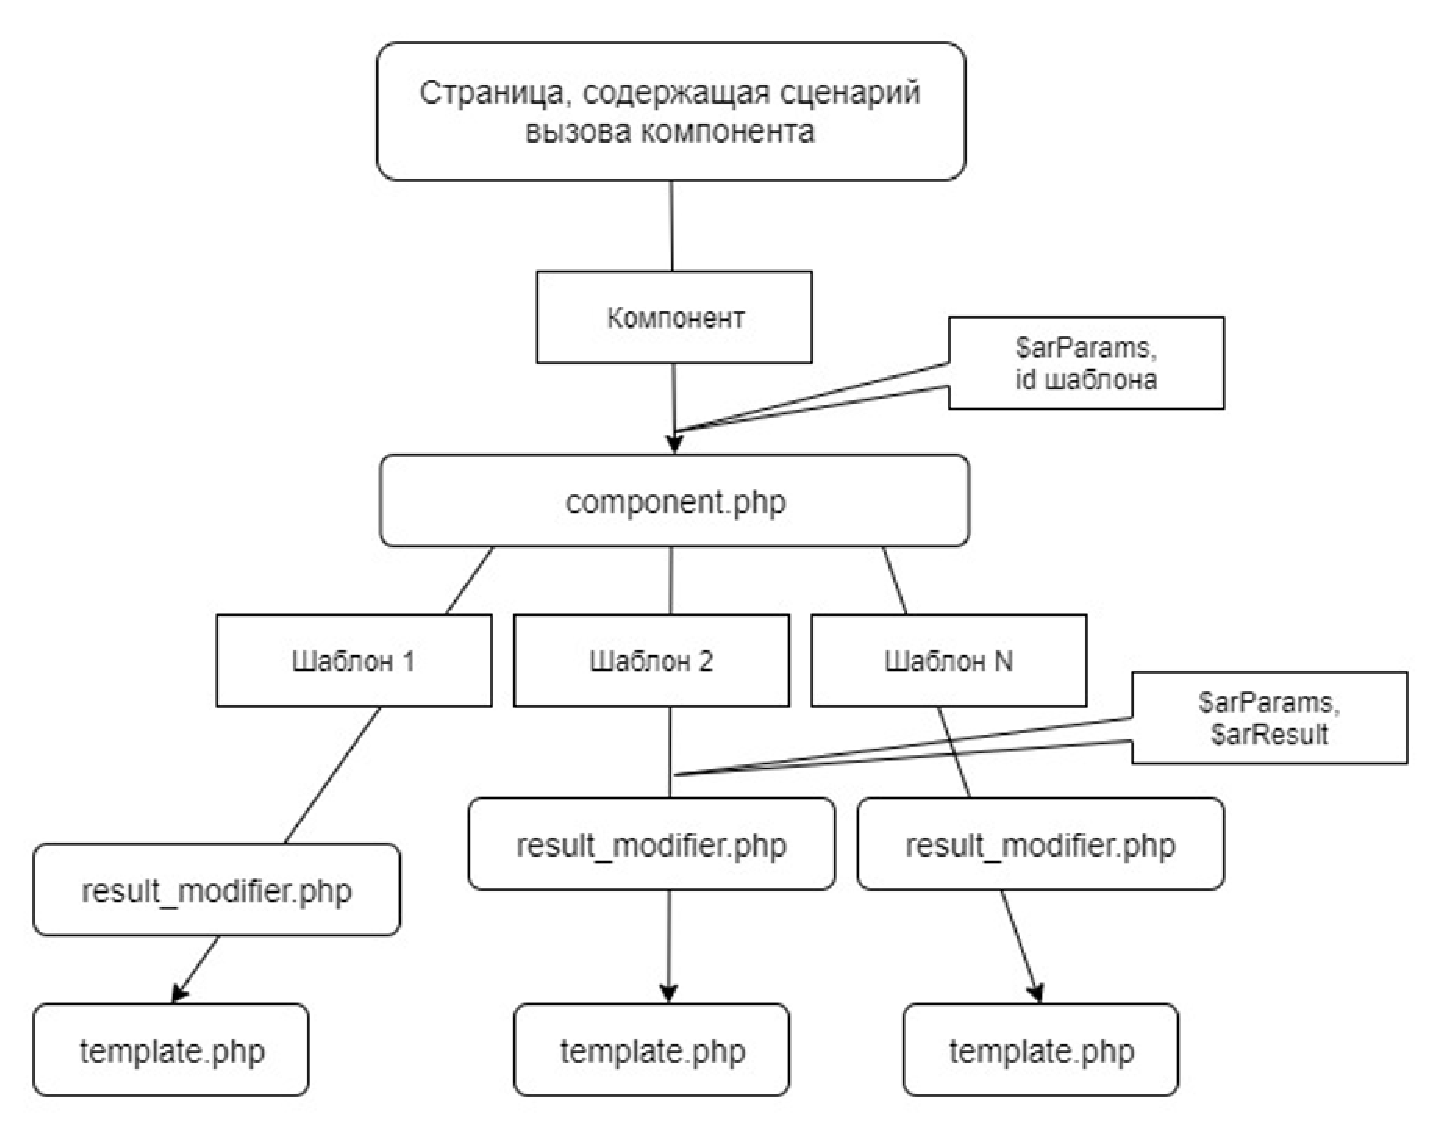
\includegraphics[width=1\linewidth]{data}}
	\caption{Диаграмма представлений}
	\label{data:image}
\end{figure}

В файле server.py написан код, который представляет собой простое веб-приложение на Python, использующее фреймворк WSGI (Web Server Gateway Interface).

Здесь импортируются различные библиотеки, классы и функции, которые используются в приложении, такие как CGI, Waitress для веб-сервера, различные представления (views) и функции для работы с файлами и базой данных. Словарь urls соотносит URL-пути с соответствующими представлениями. Когда приходит запрос, код использует этот словарь для определения, какой обработчик использовать для данного URL. Основная функция app обрабатывает POST запрос для загрузки файла, извлекает данные из формы, вставляет изображение в БД и возвращает ответ в формате JSON. Обработка GET запроса происходит с логики определения и вызова соответствующего представления и логики для обработки статических файлов, определение MIME-типа и кодировки для ответа, а также установка заголовков ответа и возврат данных в ответе.

\subsection{Диаграмма размещения}

Диаграмма размещения (рис. 3.2) отражает физические взаимосвязи между методами и представлениями.

\begin{figure}[ht]
	\center{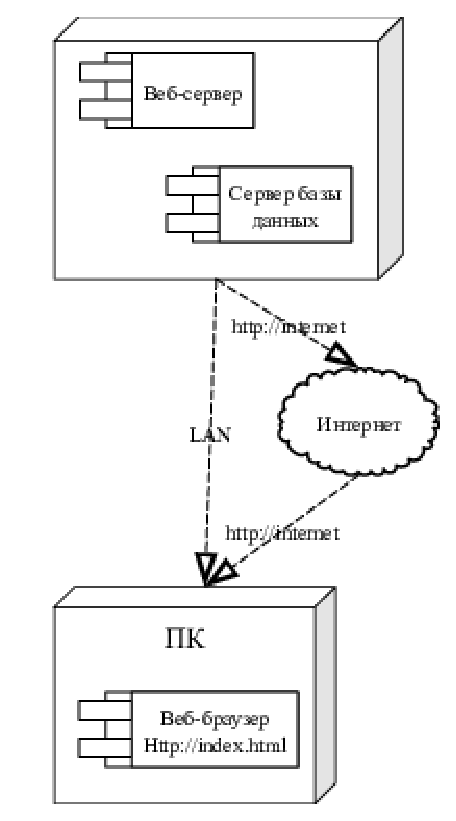
\includegraphics[width=0.57\linewidth]{place}}
	\caption{Диаграмма размещения}
	\label{place:image}
\end{figure}

Она является хорошим средством для показа маршрутов перемещения объектов и компонентов в распределенной системе.

\subsection{Содержание информационных блоков. Основные сущности}

Проанализировав требования, можно выделить две основных сущности:
\begin{itemize}
	\item "<Пользователь">;
	\item "<Добавление фотографии">;
\end{itemize}

В состав сущности "<Пользователь"> можно включить атрибуты, представленные в таблице 3.1.

\begin{xltabular}{\textwidth}{|l|l|p{1.7cm}|X|}
	\caption{Атрибуты сущности "<Пользователь">\label{news:table}}\\ \hline
	\centrow Поле & \centrow Тип & \centrow Обяза\-тельное & \centrow Описание \\ \hline
	\thead{1} & \thead{2} & \centrow 3 & \centrow 4 \\ \hline
	\endfirsthead
	\thead{1} & \thead{2} & \centrow 3 & \centrow 4 \\ \hline
	\finishhead
	id & ObjectId & true & Уникальный идентификатор \\ \hline 
	login & String & true & Логин \\ \hline 
	password & String & true & Пароль \\ \hline 
\end{xltabular}

В состав сущности "<Добавление фотографии"> можно включить атрибуты, представленные в таблице 3.2.

\begin{xltabular}{\textwidth}{|l|l|p{1.7cm}|X|}
	\caption{Атрибуты сущности "<Добавление фотографии">\label{news:table}}\\ \hline
	\centrow Поле & \centrow Тип & \centrow Обяза\-тельное & \centrow Описание \\ \hline
	\thead{1} & \thead{2} & \centrow 3 & \centrow 4 \\ \hline
	\endfirsthead
	\thead{1} & \thead{2} & \centrow 3 & \centrow 4 \\ \hline
	\finishhead
	id & ObjectId & true & Уникальный идентификатор \\ \hline 
	imagename & String & true & Название фото \\ \hline 
	imagedesc & String & true & Описание фото \\ \hline 
	imagecountry & String & true & Страна, где сделано фото \\ \hline 
	image & LONGBLOB & true & Фото \\ \hline 
\end{xltabular}

\ifПрактика{}\else{
   \section{Рабочий проект}
\subsection{Классы, используемые при разработке сайта}

Можно выделить следующий список классов и их методов, использованных при разработке web-приложения (таблица \ref{class:table}). Пример таблицы с уменьшенным межстрочным интервалом.

\renewcommand{\arraystretch}{0.8} % уменьшение расстояний до сетки таблицы
\begin{xltabular}{\textwidth}{|X|p{2.5cm}|>{\setlength{\baselineskip}{0.7\baselineskip}}p{4.85cm}|>{\setlength{\baselineskip}{0.7\baselineskip}}p{4.85cm}|}
\caption{Описание классов Bitrix, используемых в приложении\label{class:table}}\\
\hline \centrow \setlength{\baselineskip}{0.7\baselineskip} Название класса & \centrow \setlength{\baselineskip}{0.7\baselineskip} Модуль, к которому относится класс & \centrow Описание класса & \centrow Методы \\
\hline \centrow 1 & \centrow 2 & \centrow 3 & \centrow 4\\ \hline
\endfirsthead
\caption*{Продолжение таблицы \ref{class:table}}\\
\hline \centrow 1 & \centrow 2 & \centrow 3 & \centrow 4\\ \hline
\finishhead
CMain & Главный модуль & CMain – главный класс страницы web-приложения. После одного из этапов по загрузке страницы в сценарии становится доступным инициализированный системой объект данного класса с именем \$APPLICATION & void ShowTitle(string property\_code = «title», bool strip\_tags = true)
Выводит заголовок страницы
void SetTitle(string title)
Устанавливает заголовок страницы

void ShowCSS(bool external = true, bool XhtmlStyle = true)
Выводит таблицу стилей CSS страницы\\
\hline CFile & Главный модуль & CFile – Класс для работы с файлами и изображениями & array GetFileArray (int file\_id)
Метод возвращает массив, содержащий описание файла (путь к файлу, имя файла, размер) с идентификатором file\_id
\end{xltabular}
\renewcommand{\arraystretch}{1.0} % восстановление сетки

\subsection{Модульное тестирование разработанного web-сайта}

Модульный тест для класса User из модели данных представлен на рисунке \ref{unitUser:image}.

\begin{figure}[ht]
\begin{lstlisting}[language=Python]
from django.test import TestCase
from .models import *
User = get_user_model()


class ShpoTestCases(TestCase):

    def setUp(self) -> None:
        self.user = User.objects.create(username='testtestovich', password='testtestovich', first_name='Sad', last_name='')

    def test_2(self):

        self.assertEqual(self.user.first_name, 'Sad')
        self.assertEqual(self.user.last_name, 'Cat')
        print((self.user))
        print((self.user.first_name))
        print((self.user.last_name))
\end{lstlisting}  
\caption{Модульный тест класса User}
\label{unitUser:image}
\end{figure}

\subsection{Системное тестирование разработанного web-сайта}

На рисунке \ref{main:image} представлена главная страница сайта «Русатом – Аддитивные технологии».
\newpage % при необходимости можно переносить рисунок на новую страницу
\begin{figure}[H] % H - рисунок обязательно здесь, или переносится, оставляя пустоту
\center{
\includegraphics[width=1\linewidth]{main1}}
\center{\includegraphics[width=1\linewidth]{main2}}
\center{\includegraphics[width=1\linewidth]{main3}}
\caption{Главная страница сайта «Русатом – Аддитивные технологии»}
\label{main:image}
\end{figure}

На рисунке \ref{menu:image} представлен динамический вывод заголовков, включающий в себя искомые фразы при поиске фраз.

\begin{figure}[ht]
\center{
\includegraphics[width=1\linewidth]{menu}}
\caption{Динамический вывод заголовков}
\label{menu:image}
\end{figure}

На рисунке \ref{enter:image} представлен ввод данных для публикации новости.

\begin{figure}[ht]
\center{
\includegraphics[width=1\linewidth]{enter}}
\caption{Ввод данных для публикации очень-очень длинной, интересной и полезной новости}
\label{enter:image}
\end{figure}

   \section*{ЗАКЛЮЧЕНИЕ}
\addcontentsline{toc}{section}{ЗАКЛЮЧЕНИЕ}

Преимущества аддитивных технологий заключается в разнообразии процессов, позволяющих применять их в различных областях производства. Существенным ограничением же является и экономическая составляющая, которая не позволит внедрить аддитивное производство повсеместно.
  
Компании, видя, как развиваются информационные технологии, пытаются использовать их выгодно для своего бизнеса, запуская свой сайт для того, чтобы заявить о своем существовании, проинформировать потенциального клиента об услугах или продуктах, которые предоставляет. 
Для продвижения компании «Русатом – Аддитивные технологии» был разработан веб-сайт на основе системы «1С-Битрикс: Управление сайтом».

Основные результаты работы:

\begin{enumerate}
\item Проведен анализ предметной области. Выявлена необходимость использовать 1С-Битрикс.
\item Разработана концептуальная модель web-сайта. Разработана модель данных системы. Определены требования к системе.
\item Осуществлено проектирование web-сайта. Разработана архитектура серверной части. Разработан пользовательский интерфейс web-сайта.
\item Реализован и протестирован web-сайт. Проведено модульное и системное тестирование.
\end{enumerate}

Все требования, объявленные в техническом задании, были полностью реализованы, все задачи, поставленные в начале разработки проекта, были также решены.

Готовый рабочий проект представлен адаптивной версткой сайта. Сайт находится в публичном доступе, поскольку опубликован в сети Интернет.  

}\fi
\addcontentsline{toc}{section}{СПИСОК ИСПОЛЬЗОВАННЫХ ИСТОЧНИКОВ}

\begin{thebibliography}{9}

    \bibitem{javascript} Фримен, А. Практикум по программированию на JavaScript / А. Фримен. – Москва~: Вильямс, 2013. – 960 с. – ISBN 978-5-8459-1799-7. – Текст~: непосредственный.
    \bibitem{python} Бретт, М. Python и MySQL. Исчерпывающее руководство / М. Бретт. – Санкт-Петербург : Питер, 2016. – 544 с. – ISBN 978-5-496-01049-8. – Текст~: непосредственный.
    \bibitem{css} Веру, Л. Секреты CSS. Идеальные решения ежедневных задач / Л. Веру. – Санкт-Петербург : Питер, 2016. – 336 с. – ISBN 978-5-496-02082-4. – Текст~: непосредственный.
    \bibitem{mysql}	Гизберт, Д. Python и MySQL / Д. Гизберт. – Москва~: НТ Пресс, 2013. – 320 с. – ISBN 978-5-477-01174-2. – Текст~: непосредственный.
	\bibitem{html5}	Голдстайн, А. HTML5 и CSS3 для всех / А. Голдстайн, Л. Лазарис, Э. Уэйл. – Москва~: Вильямс, 2012. – 368 с. – ISBN 978-5-699-57580-0. – Текст~: непосредственный.
	\bibitem{htmlcss}	Дэкетт, Д. HTML и CSS. Разработка и создание веб-сайтов / Д. Дэкетт. – Москва~: Эксмо, 2014. – 480 с. – ISBN 978-5-699-64193-2. – Текст~: непосредственный.
	\bibitem{bigbook}	Макфарланд, Д. Большая книга CSS / Д. Макфарланд. – Санкт-Петербург : Питер, 2012. – 560 с. – ISBN 978-5-496-02080-0. – Текст~: непосредственный.
	\bibitem{uchiru}	Лоусон, Б. Изучаем HTML5. Библиотека специалиста / Б. Лоусон, Р. Шарп. – Санкт-Петербург : Питер, 2013 – 286 с. – ISBN 978-5-459-01156-2. – Текст~: непосредственный.
	\bibitem{chaynik}	Титтел, Э. HTML5 и CSS3 для чайников / Э. Титтел, К. Минник. – Москва~: Вильямс, 2016 – 400 с. – ISBN 978-1-118-65720-1. – Текст~: непосредственный.    
	\bibitem{22}	Титтел, Э. HTML5 и CSS3 для чайников / Э. Титтел, К. Минник. – Москва~: Вильямс, 2016 – 400 с. – ISBN 978-1-118-65720-1. – Текст~: непосредственный.    
	\bibitem{1231}	Титтел, Э. HTML5 и CSS3 для чайников / Э. Титтел, К. Минник. – Москва~: Вильямс, 2016 – 400 с. – ISBN 978-1-118-65720-1. – Текст~: непосредственный.    
	\bibitem{sdf}	Титтел, Э. HTML5 и CSS3 для чайников / Э. Титтел, К. Минник. – Москва~: Вильямс, 2016 – 400 с. – ISBN 978-1-118-65720-1. – Текст~: непосредственный.    
	\bibitem{servsssds}	Титтел, Э. HTML5 и CSS3 для чайников / Э. Титтел, К. Минник. – Москва~: Вильямс, 2016 – 400 с. – ISBN 978-1-118-65720-1. – Текст~: непосредственный.
\end{thebibliography}

\ifВКР{\appendix{Представление графического материала}

Графический материал, выполненный на отдельных листах,
изображен на рисунках А.1--А.\arabic{числоПлакатов}.
\setcounter{числоПлакатов}{0}

\renewcommand{\thefigure}{А.\arabic{figure}} % шаблон номера для плакатов

\begin{landscape}

\begin{плакат}
    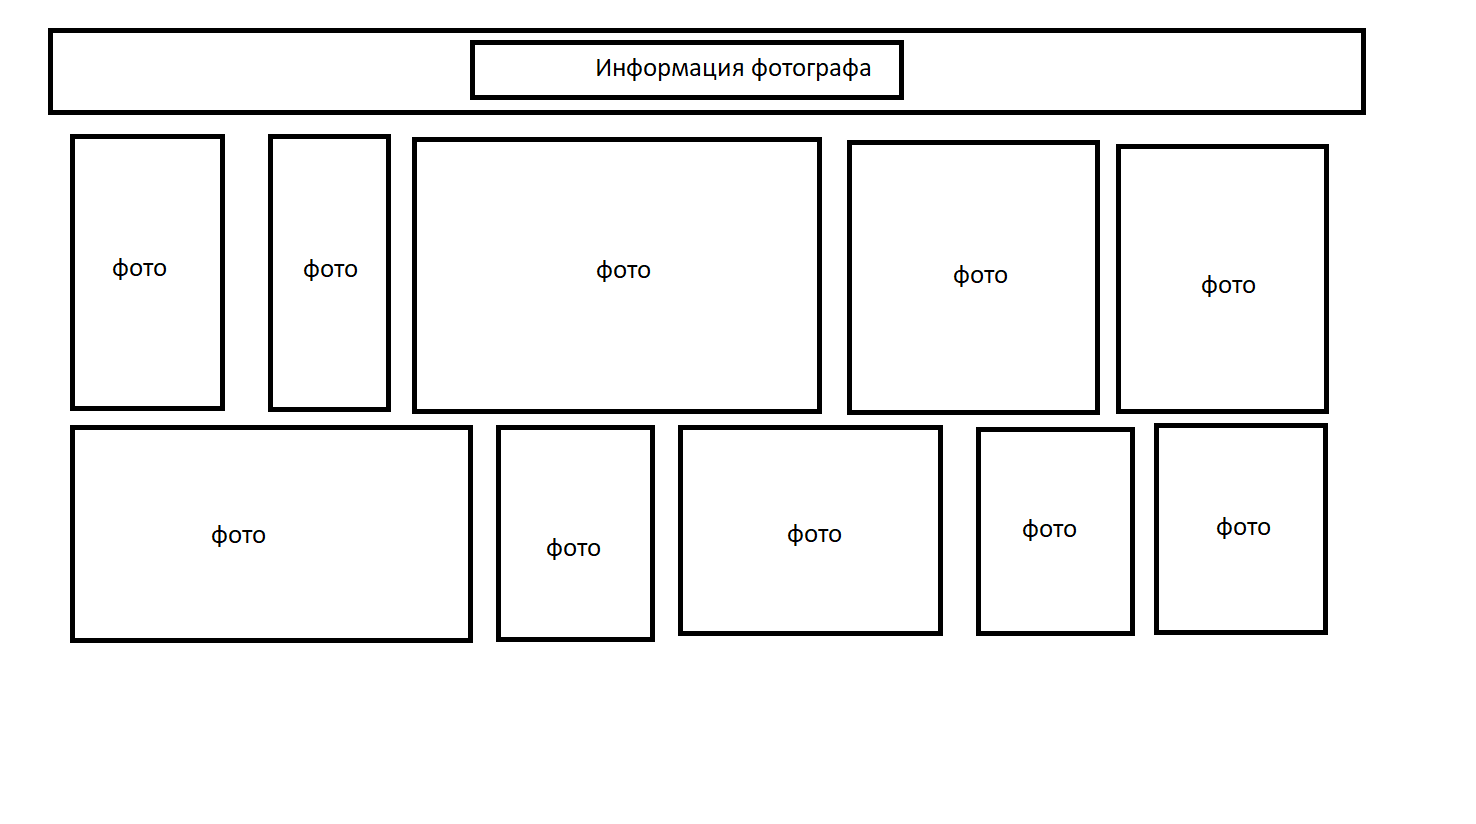
\includegraphics[width=0.82\linewidth]{плакат1.png}
    \заголовок{Сведения о ВКРБ}
    \label{pl1:image}      
\end{плакат}

\begin{плакат}
    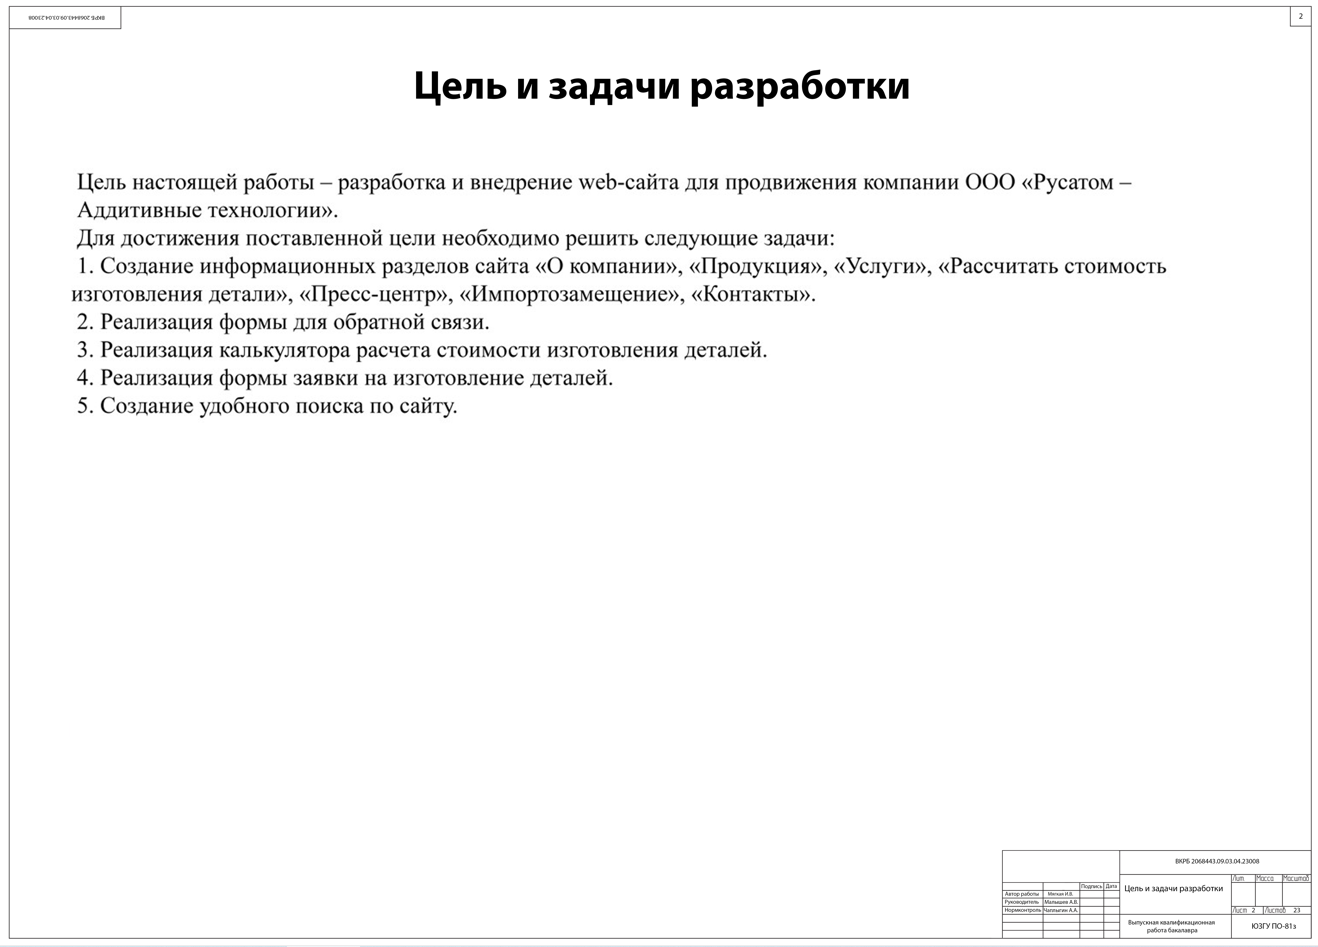
\includegraphics[width=0.82\linewidth]{плакат2.png}
    \заголовок{Цель и задачи разработки}
    \label{pl2:image}      
\end{плакат}

\begin{плакат}
    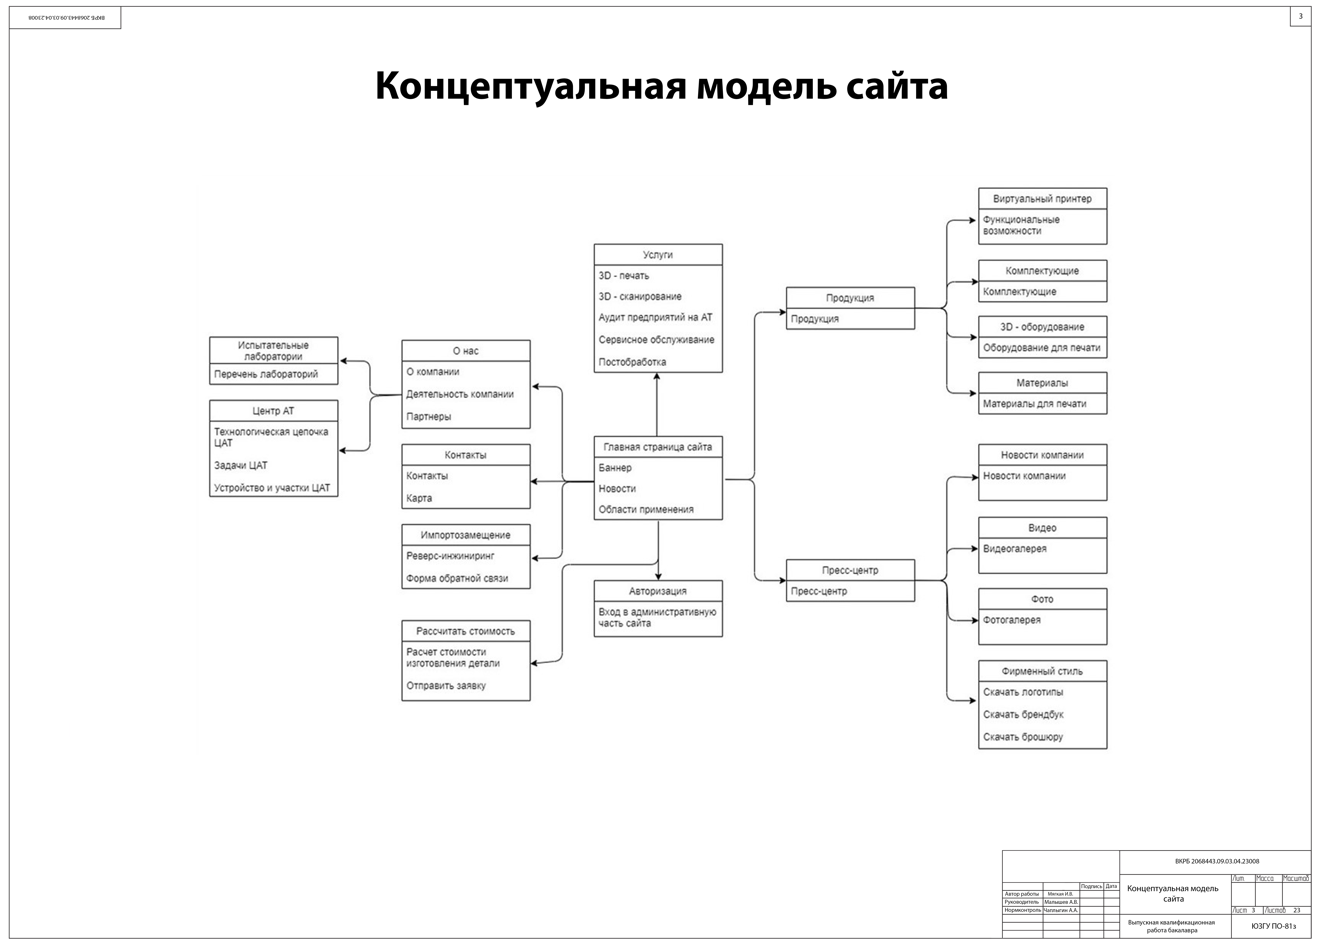
\includegraphics[width=0.82\linewidth]{плакат3.png}
    \заголовок{Концептуальная модель сайта}
    \label{pl3:image}      
\end{плакат}

\begin{плакат}
    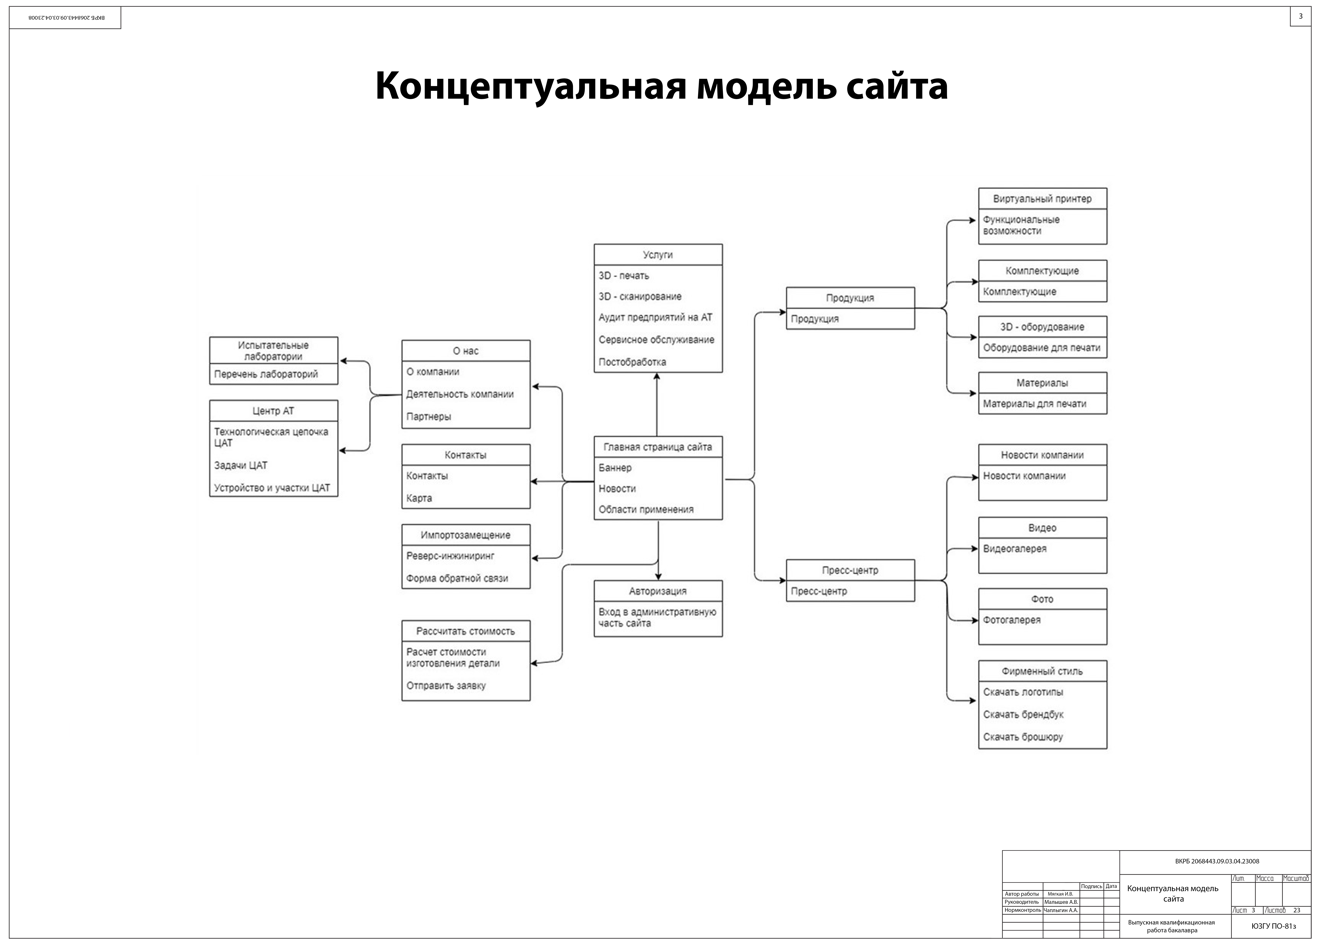
\includegraphics[width=0.82\linewidth]{плакат3.png}
    \заголовок{Еще плакат}
    \label{pl4:image}      
\end{плакат}

\end{landscape}
}\fi
\ifПрактика{}\else{\appendix{Фрагменты исходного кода программы}

main.tex
\lstinputlisting[language=Tex, frame=none]{main.tex}

ТехПроект.tex
\lstinputlisting[language=Tex, frame=none]{ТехПроект.tex}

\ifВКР{
\newpage
\addcontentsline{toc}{section}{На отдельных листах (CD-RW в прикрепленном конверте)}
\begin{center}
\textbf{Место для диска}
\end{center}
}\fi
}\fi
\end{document}
